\chapter{Statistical Process Control- SPC}
\label{sec:spc}

Statistical process control deals with the quantitative analysis of a ``process'', which may be a production line, a service, or any other repeated operation.
As such, it may be found in the Analyze, Improve, and Control stages of the DMAIC cycle.
The purpose of the SPC, in the terms coined by Shewart, is to seperate the variability in the process into \emph{assignable} causes of variation and \emph{chance} causes of variation.\marginnote{Causes of variation}
These are also known as \emph{special} and \emph{common} causes of variation, respectively. 
A process is said to be in \emph{statistical control} if all its variation is attributable to chance causes.
If this is not the case, we call it \emph{out of control} and we will seek the assignable causes, remove then, and   re-analyze.


All the previously mentioned statistical tools may be called upon for this analysis. 
In the context of process control, a subset of tools has gained the nick-name ``The Magnificent Seven''. These include:
\begin{description}
\item Histogram and stem-and-leaf plot. As described in Chapter~\ref{sec:exploratory}.
\item Check Sheet. [TODO: add figure]
\item Pareto chart. An ordered bar plot of the events due to the various assignable variability causes. [TODO: add figure]
\item Cause-and-effect diagram. A visualization of candidate assignable variability causes. [TODO: add figure]
\item Defect concentration diagram. A visual inspection of the location of defects on the product. 
\item Scatter plot. As described in Chapter~\ref{sec:exploratory}.
\item Control chart. A powerful analysis tool to which we devote the rest of this chapter. 
\end{description}





%\begin{pgfpicture}
%    \pgftext{\pgfimage[width=0.6\linewidth, height=0.3\textheight]{}}
%\end{pgfpicture}


\section{A soft start. The \barxChart}


% basic idea
% descion variables: sample size, intervals, statistic, limits, rational groupins, type I error rate, multiple criteria
% phase I and II.
% what to do in case of alarm?
% extensions: probability limits, other statisics=, sample , adaptive parameters, other rules, non normality, variable sample size, moving windows
% considerations for setting these values.
% Setting limits: history, bootstrap, CLT
% multiplicity in control charts
% FDR controlling limits
% western electric rules. The type I error probability of the rule.
% nelson rules


We demonstrate the concepts and utility of Control Charts with the simplest, yet most popular of them all, the \barxChart. 
The chart borrows its name from the fact that it is essentially a visualization of the time evolution of the average ($\bar{x}$) of the CTQ of a sample of products. 
The chart is also augmented with visual aids that help in determining if the process is \emph{in control}, i.e., if it consistent with its own history. 
Process capability analysis may benefit from the ideas of control charts. We emphasize however, that control charts have no information on the specifications of the process, merely on its own history.

An illustration of a \barxChart is given in Figure~\ref{fig:bar_x_chart}. 
The ingredients of this chart is the centerline, the control limits, and $\bar{x}$ evolving in time. 
If at each period $t=1,\dots,\tau$, we compute the average of $n$ samples, we denote $\bar{x}_t:=1/n \sum_{i=1}^n x_{it}$.

\begin{figure}[h]
\centering
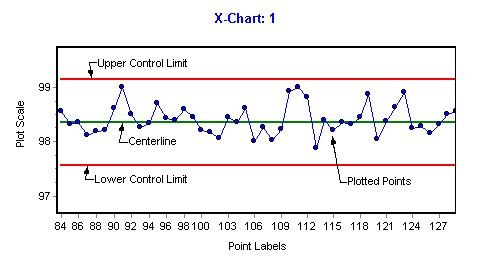
\includegraphics[height=0.3\textheight]{art/X-chartExample}
\caption[\barxChart]{\barxChart. \newline \url{https://mvpprograms.com/help/P-mvpstats/spc/WhatAreControlCharts}}
\label{fig:bar_x_chart}
\end{figure}






Figure~\ref{fig:bar_x_chart} makes it evident \barxChart requires several design decisions.
A standard design decision is setting the center line as the grand average of the process: 
\begin{align}
\label{eq:centerline}
	1/\tau \sum_{t=1}^\tau \bar{x}_t
\end{align}


If it is unclear to you, how may we compute the grand average of a process that is still evolving and has not finished, you are right! We thus introduce the ideas of \emph{Phase I} and \emph{Phase II}. \marginnote{Phase I/II}
Initially we assume the process it out of control, we identify and remove assignable causes of variation, until we are left with a ``well-behaved'' subset of data points. We call this Phase I, and we use it to initialize required quantities such as the centre line. 
Eq.(\ref{eq:centerline}) thus implies that in Phase I we were left with $\tau$ samples assumingly in statistical control.
After the chart has been calibrated, and major assignable sources of variability removed, we can focus on monitoring the process, known as Phase II.


Other design decisions to be made are:
\begin{enumerate}
\item UCL and LCL \footnote{Do not confuse with USL and LSL!}.
\item Sample size in each sample.
\item Rational groupings (within-period sampling scheme).
\item Frequency of samples (between-period sampling scheme). 
\end{enumerate}
These deign decisions ultimately govern the error rate (false positive rate) and power (false negative rate) of the chart, which in turn, incur some financial costs. 
For now we will restrict attention to type I/II error rates, until Section~\ref{sec:economical_considerations} where we consider these choices as economical optimization problems.

For ease of exposition, control chart design is demonstrated for the \barxChart, but equally apply to other control charts.
We start by a type I error rate analysis. 
Denote $\alpha_t$ the false alarm probability at period $t$.
How do our design choices affect $\alpha_t$?
\begin{align}
	\alpha_t &:= 1-P(\bar{x}_t \in [UCL,LCL]) \\
	&= 2 P(\bar{x}_t<UCL) \\
	&= 2 P(Z<\frac{UCL-\mu}{\sigma_{\bar{x}}}) \\
	&= 2 P(Z < -k) \\
	&= 2 \Phi(-k)
\end{align}
The above follows from assuming that $UCL:=\mu + k \sigmabar, LCL:= \mu - k \sigmabar$, $\x_{it}\sim \gauss{\mu,\sigma}$, and denoting $\sigmabar:= \frac{\sigma}{n}$.
A typical design choice is $k=3$, known as \emph{3-sigma control limits}, implying a false alarm rate of $\alpha_t=0.0027$.\marginnote{3-Sigma Control Limits}
Since we assumed the process is fixed over time, then so is $\alpha_t$ and we can simply write $\alpha$.

A power analysis for our design choices follows the same lines.
Denote $\beta_t$, and $\pi_t=1-\beta_t$ the type II error rate, and power, at period $t$.
We then have


Another important related quantity is the \emph{average run length} (ARL), which is the number of periods between two crossings of control limits. 



\section{Other Control Statistics}
\subsection{$R$ Chart}
\subsection{$s$ Chart}
\subsection{$s^2$ Chart}
\subsection{Shewhart Individuals Control Chart}
\subsection{Three-way Chart}
\subsection{$p$ Chart}
\subsection{$np$ Chart}
\subsection{$c$ Chart}
\subsection{$u$ Chart}
\subsection{Time Series Model}
\subsection{Regression Control Chart}



\section{Running Window Charts}
\subsection{$EWMA$ Chart}
\subsection{$Cumsum$ Chart}

\section{Economical Design of Control Charts}
\label{sec:economical_considerations}


\section{Multivariate Control Charts}
% Wishart
% Srivastava Du
% PCA
% Higher criticism



\subsection{Non-Statistical Target Functions}





